\documentclass[a4paper,12pt]{article}

\usepackage[]{geometry} %textwidth=6.5in,textheight=9in
\usepackage{graphicx}
\usepackage{graphics}
\usepackage{amsmath}
\usepackage{url}
\usepackage{float}
\usepackage{hyperref}
\usepackage{listings}
\usepackage{minted}
\usepackage{pdflscape}
\usepackage{rotating}
\usepackage{mdframed}

\hypersetup{ colorlinks=true, linkcolor=blue, filecolor=magenta, urlcolor=cyan }
\renewcommand\listoflistingscaption{List of source codes}

\begin{document}

\begin{titlepage}
	\begin{center}
		%\vspace*{1cm}
		\huge
		\textbf{Examiner's report\\}
		\vspace{0.5cm}
		\Large
		Machine Learning in Drug Discovery and Design \\
		\vspace{1.5cm}
		\textbf{Ibraheem Ajibola Ganiyu}
		\vfill
		\textsc{12844772} \\
		BSc. (Hons) Software Engineering. \\
		\vspace{0.8cm}
		\large
		School of Computing, Engineering and Mathematics \\
		University of Brighton \\
		\date{\today}
	\end{center}
\end{titlepage}

\pagenumbering{roman}
\tableofcontents
\newpage
%\listoffigures
%\listoftables
%\listoflistings
%\newpage
\pagenumbering{arabic}

\section{Project Evaluation}
	The title of my dissertation was \textit{Machine Learning in Drug Discovery and Design} with the main focus being on predicting the penetration of drugs into the blood brain barrier.
	
	%How it fits into the modules studies
	It is a research based project that is inspired by my placement spent at AstraZeneca, a bio-pharmaceutical company, where I gained practical experience in software development for clinical trials and research based tasks. The project draws on the knowledge I have gained from my programming modules in the second year and also my final year module \textit{CI346 Programming Languages and Client-Server Computing} and also the research skills I have gained both at the university and at AstraZeneca.
	
	%Significant area of project work
	A significant amount of the time spent on the project was used to learn the necessary techniques needed to perform machine learning on large datasets and also on the required chemoinformatics knowledge required to successfully complete the project.
	
\section{Background Research}
	I conducted research into Artificial Intelligence especially Machine Learning before embarking on the project. With little real world knowledge on how to perform machine learning, I turned to machine learning texts such as \textit{Machine Learning by Tom Mitchell} and \textit{Artificial Intelligence: A Modern approach by Peter Norvig}. 
	
	For the implementation of the machine learning algorithms, I also researched and experimented with numerous machine learning libraries but eventually settled on the Scikit-Learn and RDKit software libraries, due to their popularity and ease of use for data science. I also read \textit{Chemoinformatics: Concepts, Methods and Tools for Drug Discovery} to get the necessary chemistry knowledge I needed to successfully work with the dataset.
	
\section{Methodology and Planning}
	%Include original plan and compare any changes
	As the project is a research based one, the core requirements or experiments were established before the project life cycle began. The core requirement of the project was to build a machine learning classifier that could be trained with our dataset on how to predict the probabilities of drugs passing through the blood brain barrier. As stated in the interim report, the main stages of the implementation phase with deliverables of the projects are
		\begin{itemize}
			\item Data Cleaning
			\item Classifier Training
			\item Ensemble Classifier training
			\item Deployment 
			\item Testing and Quality Assurance
		\end{itemize}
	\subsection{Detailed discussion the project stages}
		\subsubsection{Data Cleaning}
		As is the norm for most data science tasks, the dataset needed to be parsed, unnecessary data removed and the required portions transformed into another form for use. 
		\subsubsection{Classifier and Ensemble Classifier Training}
		Arguably one of the most important sections, the respective machine learning classifiers chosen, needed to be trained with the processed dataset. Here, four machine learning classifiers (K-Nearest Neighbours, Support Vector Machines, Random Forests and Neural Networks) were trained. In the original project plan, deep neural networks were scheduled to be trained with the dataset but this couldn't be done due to time constraints.\\
		All the trained classifiers were then combined successfully into an Ensemble classifier with an average accuracy of $87\% (+/- 7\%)$.
		\subsubsection{Deployment}
		In the interim report, it was stated that the project would yield 3 deliverables: a web client, a web server and a prediction API (engine). The ensemble classifier was successfully wrapped in a web server and a REST API was exposed to receive and return prediction results. A web client, however, was not built; This was noted down as an extension that would be done given enough time as it would provide an intuitive and easy accessible UI to make the product easier to use.
		\subsubsection{Testing and Quality Assurance}
		All the classifiers were tested using the standard cross validation technique for evaluating machine learning classifiers and an ROC (Receiver Operating Characteristic) curve was drawn to compare the ensemble classifier against a dummy classifier that is making random guesses.
	

\section{Research Evaluation}
	%Progress made
	The core of the research was to build a classifier to predict the probability of a potential drug candidate passing through the blood brain barrier. This was successfully achieved with an Ensemble classifier that performs at best with an accuracy of 94\% and at worst with an accuracy of 80\%.
	
	\subsection{Problems encountered}
	One of the common problems encountered throughout the training of the classifiers was achieving accuracy scores lower than 50\% on the classifiers. A classifier achieving lower than 50\% on prediction results would achieve poorer results than a dummy classifier making random guesses. 
	
	Also, due to the high dimensional nature of the dataset it took longer to train some classifiers, especially the support vector machine classifier as based on read literature we know it would perform poorly on high dimensional dataset which it did.
	
	Another problem encountered at the beginning during the preprocessing of the dataset was the inability of RDKit to parse some SMILE formats. This is most likely due to the SMILE formats being malformed and probably due to a bug in the RDKit library. However, only a small number of molecule SMILEs, 13 , failed to be parsed. This was safely ignored as we still had 2040 molecule SMILEs left that successfully got parsed.
	
	The last problem encountered in the project was combining all the individually trained classifiers into an Ensemble classifier. An option explored was to create a custom class in python where it receives as input the feature vectors and then passes this vector to the individual classifiers and collects their results, however, this resulted in scope creep as doing such as task turned out to be much more difficult than expected. 
	
		\subsubsection{Solutions put forward}
		A solution implemented to prevent the classifiers from achieving poor results was to perform feature engineering on the input dataset. An example was the scaling of values in the dataset to have a maximum of 1 and a minimum of -1 using a \textit{MinMaxScaler}. This helped normalize the dataset as some classifiers that utilise distance metrics would return poor results due to the large variance in the dataset. Also the neural network classifier would converge much faster during gradient descent with a normalised data due to the normalisation.
		
		To help reduce the training time of the support vector machine (SVM) classifier. The Principal Component Analysis (PCA) algorithm was used on the dataset before feeding it to the SVM classifier. Different values were experimented with to the determine the best number of components to use in the SVM classifiers that would achieve the maximum result whilst still reducing the training time of the algorithm.
		
		The solution to the incompatible ensemble classifier problem was to utilise the \textit{Voting Classifier} class in Scikit-Learn. This had the advantage of being an Ensemble classifier and also had the options of specifying the voting mechanism to use. The voting mechanism here refers to the metric to use when deciding the final prediction result of the Ensemble from the results of the individual classifiers.
		
	\subsection{Assessment on the success of the project}
		%Compare your prediction accuracy to other bbb projects
		Based on the prediction accuracy of the ensemble classifier, the project could be said to be successful. In a paper by Ana Teixeira et al, \textit{A Bayesian Approach to in Silico Blood-Brain Barrier Penetration Modeling}, they listed all the accuracy of the classifiers numerous other researchers have applied to the BBB problem. The lowest result was an accuracy of 74.8\% in 2000 using the partial least-squares method whilst the highest was an accuracy of 97.2\% in 2007 using a recursive partitioning model and partial least squares method. 
		
		This project achieves an average prediction accuracy of 87\% (+/- 7\%) which lies in between the results mentioned earlier.
\section{Areas of Interest}
	%Include image of prediction result and curl call
	\subsection{Prediction API}
	The prediction API is one of the areas of the project that can provide real world value. The decision to use a REST API was to enable the integration of the Ensemble classifier into any other other program or software that the scientist uses in the form of micro-services. A sample use case would be web client that draws a list of molecules from a virtual library micro-service, the user of the client then performs some filtering on the list and sends the remaining molecules to our prediction micro-service, which then returns a list of molecules with their respective probabilities of passing through the blood brain barrier returned. An example taken from the project is shown below, where a sample curl call is made.
		\begin{minted}[obeytabs=false,tabsize=2]{bash}
		$ curl -H "Content-Type: application/json" -X POST -d 
		'{"smile":"Cn1c2CCC(Cn3ccnc3C)C(=O)c2c4ccccc14"}'   
		http://localhost:5000/api/prediction
		\end{minted}
	And a prediction result is returned as shown in figure \ref{fig:bbb_sample_prediction_result} 
		\begin{figure}[H]
			\centering
			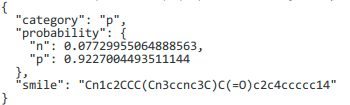
\includegraphics[width=0.6\textwidth,scale=1]{sample_prediction_result}
			\caption{Sample prediction result for the BBB Rest API}
			\label{fig:bbb_sample_prediction_result}
		\end{figure}
	\subsection{Learning curve of Ensemble classifier}
	The learning curve of the ensemble classifier is also another area of interest as shown in figure \ref{fig:learning_curve_ensemble}.
		\begin{figure}[H]
			\centering
			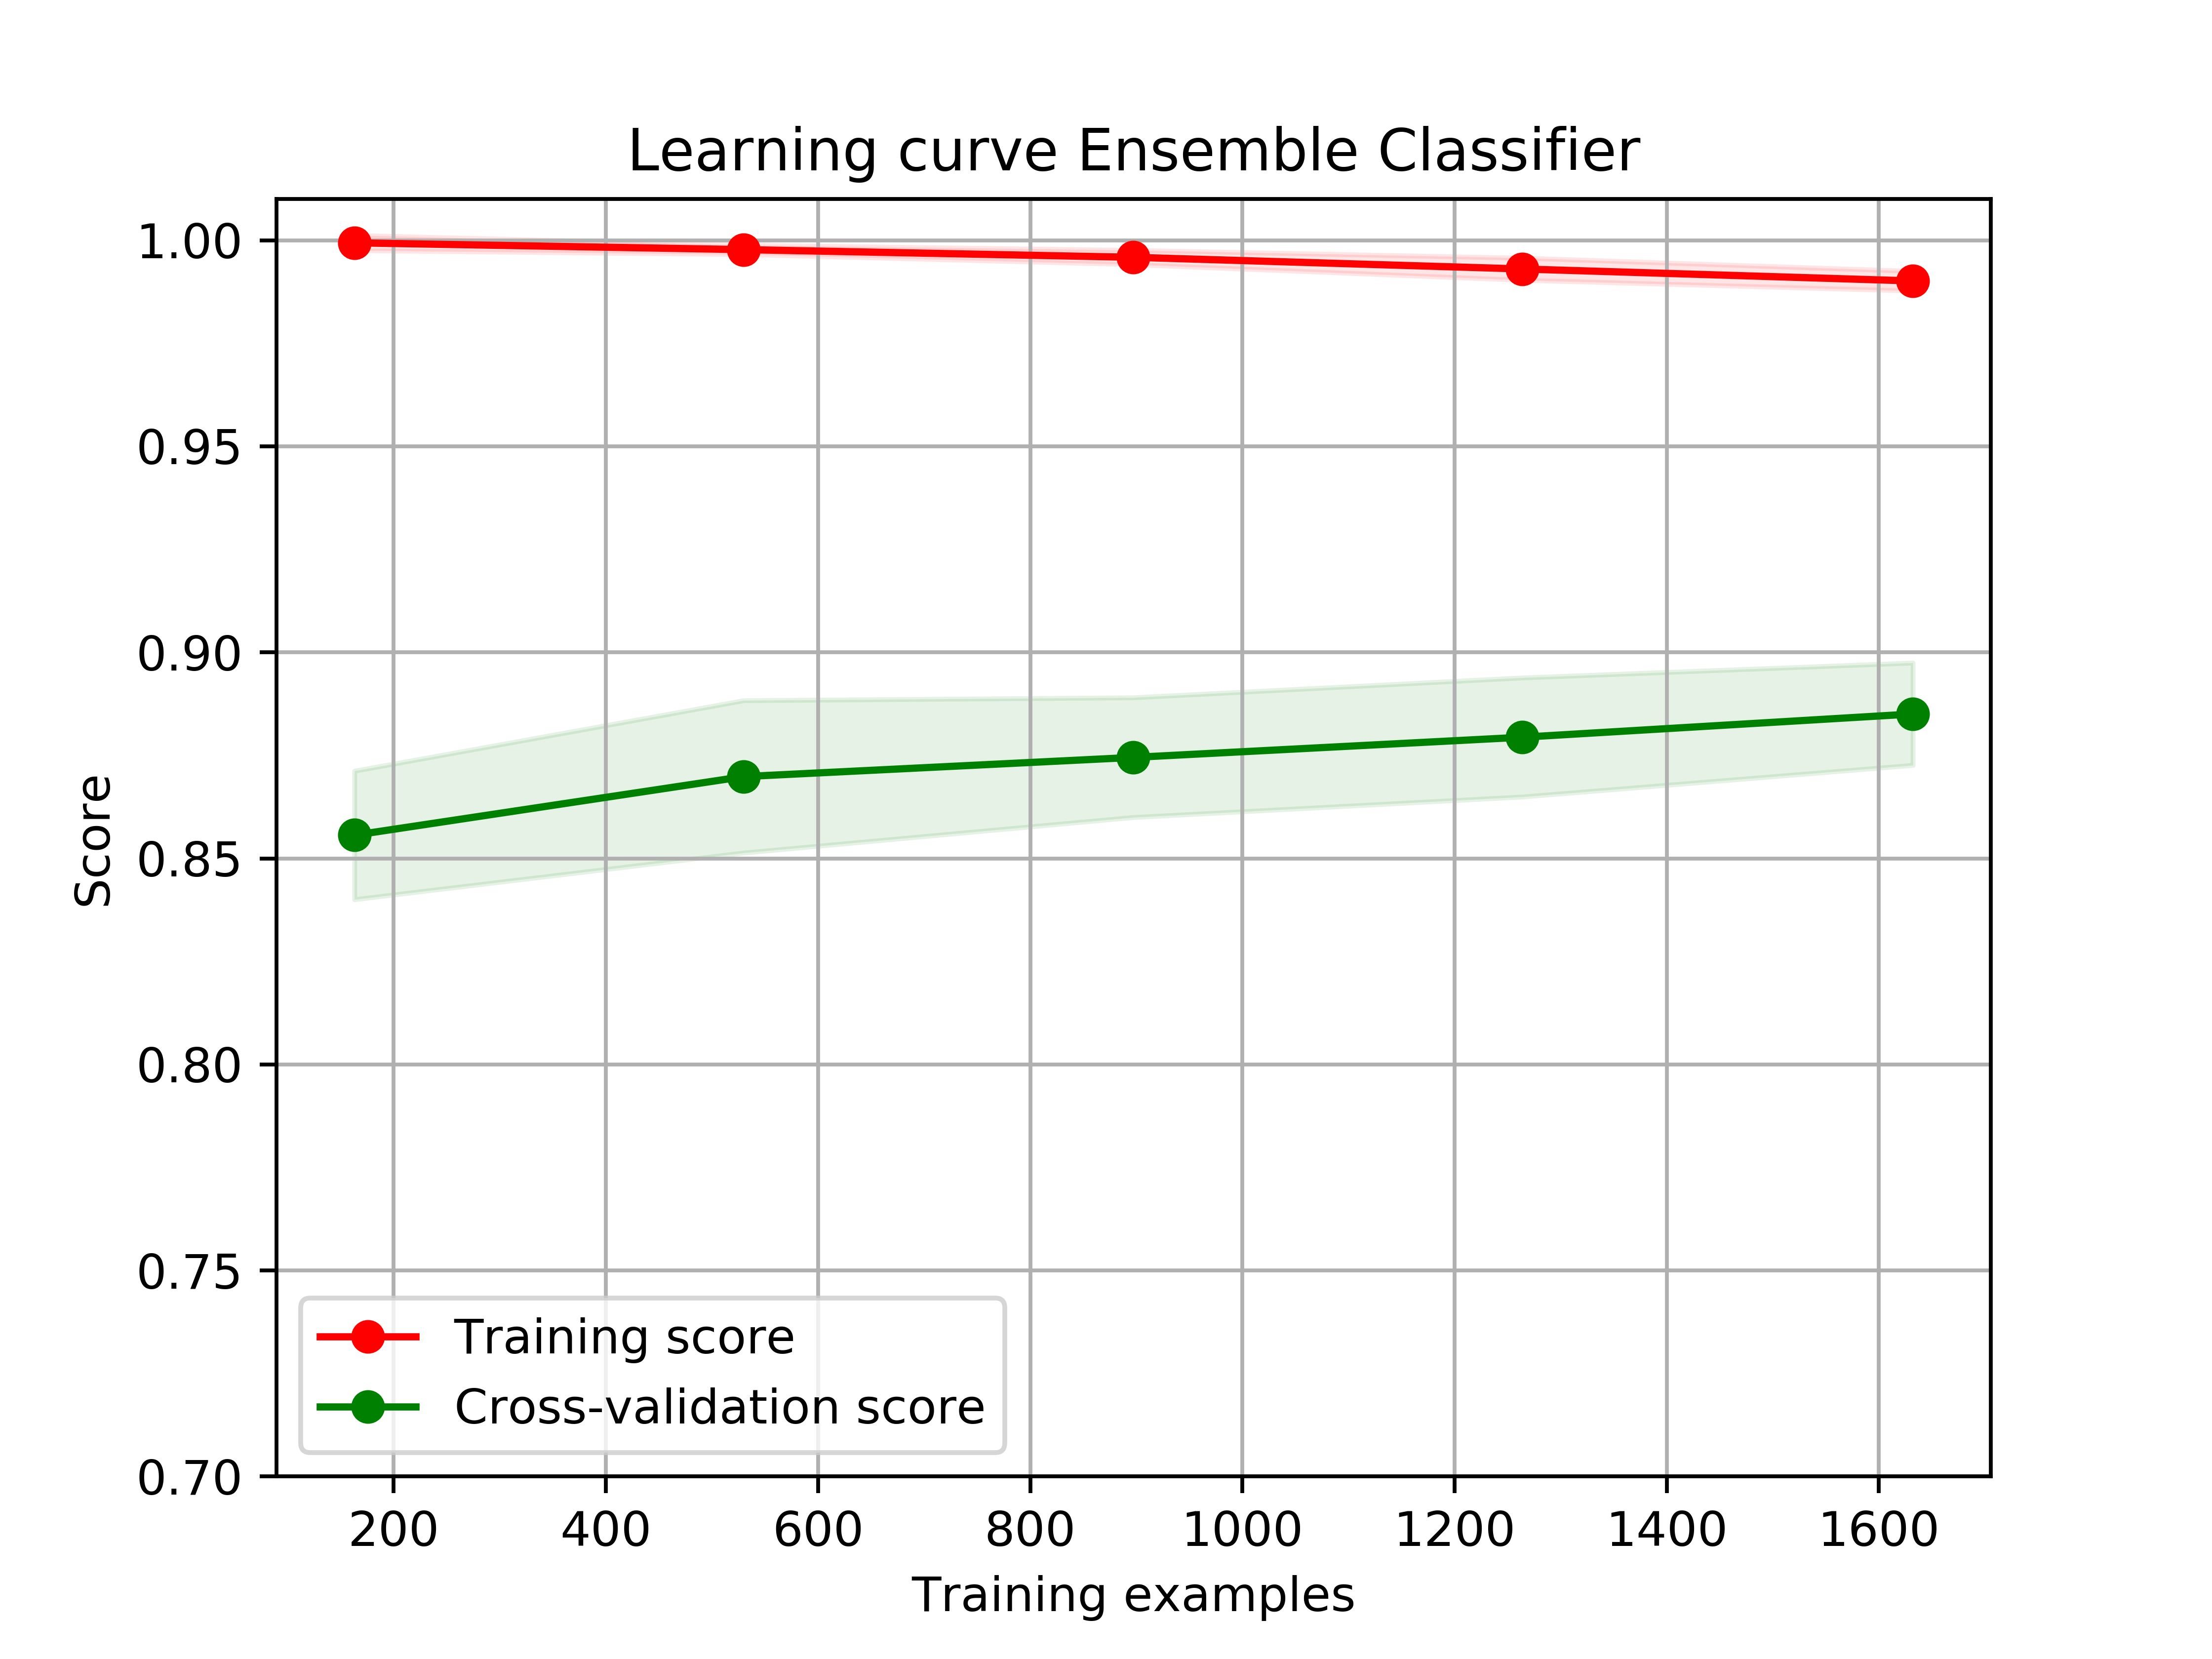
\includegraphics[width=\textwidth,scale=1]{learning_curve_ensemble_clf}
			\caption{Learning Curve for the Ensemble classifier}
			\label{fig:learning_curve_ensemble}
		\end{figure}
	The reduction in training score shows that the classifier over fits less with more data which is ideal as we want it to perform well on new datasets. The cross validation score also increases with more data, the total number of samples in the dataset was 2048; Which is a small amount of data compared to large body of chemical datasets available. The assumption here re-enforced by figure \ref{fig:learning_curve_ensemble} is that with more data, we can achieve a higher accuracy score on the ensemble classifier
	
\section{Further Areas for improvement}
	Given more time, other machine learning classifiers could have been explored, especially deep learning techniques. Based on read literature, they have found a profound and effective use in virtual screening. 
	
	Also, the total training time of the classifiers take roughly about 30 minutes. One of the proposed solutions at the beginning of the project was to implement "Map Reduce" using Apache Spark to train all the respective classifiers on different clusters and combine the result. This would greatly reduce the training time especially if dealing with a larger dataset.

\end{document}